\documentclass{jsarticle}

% パッケージ
\usepackage[dvipdfmx]{graphicx}
\begin{document}

% 脚注フォーマット
\renewcommand\thefootnote{\arabic{footnote})}


% 表紙

{\Large \today 提出}\\ % 提出日

\begin{center}
\vspace{120truept}
{\huge 平成28年度 卒業論文\\[10mm]
IPOほにゃらら}\\ % タイトル
\vspace{10truept}
{\Large サブタイトル}\\ % サブタイトル(なければコメントアウト)
\vspace{120truept}
{\huge 学籍番号 07-150041}\\ % 学籍番号
\vspace{50truept}
{\huge 東京大学経済学部経済学科\\[50truept]
岡部 匡志}\\ % 著者

\end{center}
\newpage
\begin{center}
{\Large IPOほにゃらら}\\ % タイトル
\end{center}

% 目次
\tableofcontents
\vspace{120truept}
% 本文
\section{はじめに}
本稿では、日本の新規株式公開\footnote[1]{Initial Public Offering。以下、 「IPO」とする。}市場において、直近の数社のパフォーマンスがアンダープライシング\footnote[2]{初期収益率とも。\{(初値) - (公開価格)\} / (公開価格)\} として示される。ここで、公開価格とは、「IPO直前に希望する投資家に対して新規公開予定の株式を売却する際の価格(岡村 2011\cite{okamura})」である。また、本稿では初値として、マーケットで付けられた、取引初日における最初の価格を用いる。}にどのような影響を及ぼしているのかについて考察を行う。
\section{IPOにおけるアンダープライシング}
\subsection{アノマリーとしてのアンダープライシング}
アンダープライシング自体は、国内外で一種の経済学的アノマリー\footnote[3]{例えば、辰巳・桂山 2005\cite{tatsumi}に、ファイナンス分野で知られるアノマリーが詳しい。}として知られており、表\ref{around_world}の通り、国内外でその存在が継続的に確認されている。 \par
公開価格には企業のファンダメンタルズが適切に評価されており、初値は株式市場において効率的に形成されると想定するなら、このような現象が継続的に発生しているという事実は、アノマリーと言わざるを得ない。投資家にとっては、公開価格で株式を購入し、数週間後の上場後に株式を売却するだけで、高い収益率を得られることになり、実際に、IPO時において、アンダーライター\footnote[4]{ここでは、株式の発行・売出しに際し、株式を売れ残った際に発行者や所有者から取得する者のことであり、日本国内においては、IPOを主導する主幹事証券会社を中心としたシンジゲート団のことを指す。}が実施する公募への抽選には個人投資家からの注文が殺到している状態である。

\begin{table}[t]
	\caption{世界各国における初期収益率の算術平均。
	Loughran et el.(1994, updated 2015) \cite{Loughran}より一部抜粋。}
	\label{around_world}
	\centering
	\begin{tabular}{cccc}
		\hline
		国名&サンプル数&期間&平均初期収益率(100\%からの乖離) \\
		\hline \hline
		英国&4,932&1959-2012&16.0\% \\
		韓国&1,758&1980-2014& 58.8\% \\
		シンガポール&609&1973-2013&25.8\% \\
		タイ&500&1987-2012&35.1\%\\
		台湾 &1,620 &1980-2013&38.1\% \\
		中国&2,512&1990-2013&118.4\%\\
		ドイツ&736&1978-2011&24.2\% \\
		日本&3,236&1970-2013&41.7\% \\
		フランス & 697 & 1983-2010 & 10.5\% \\
		米国&12,702&1960-2012&16.9\%\\
		\hline
	\end{tabular}
\end{table}


\subsection{アンダープライシングの決定メカニズムについての仮説}
前述した、IPOにおけるアノマリー、ある種のマーケットの歪みは、研究者や投資家たちの強い関心を集めてきた。特に研究面の関心は、アンダープライシングを合理的に説明する決定メカニズムの解明に向けられており、数多くの仮説が提案されてきた。\par
既存研究における仮説は、大きく2つに分類出来るだろう。すなわち、アノマリーの原因を情報の非対称性に求めるものと、各プレーヤーの限定合理性に求めるものである。\par
前者の仮説については、岡村 2011\cite{okamura}によく整理されている。本稿では名前を挙げるに留めるが、「逆選択回避仮説(別名:Winner's Curse)」「エージェンシー仮説」「情報検事仮説」など、それぞれ、アンダーライターが公開価格を意図的に引き下げる誘引を持つことを説明しているものである。\par

また、アンダーライターではなく、投資家の側に、公開前需要の申告\footnote[5]{後述するブックビルディング方式における公開価格決定プロセスの一部。}に際して、株式の市場価格の観察不能性によるリスクの存在から、公開価格を押し下げる誘引が存在することを説明した論文として、池田 2013\cite{ikeda}がある。\par

\begin{figure}[tbp]
  \begin{center}
  \caption{アンダープライシングの年度別平均値の推移(1997〜2017)}
    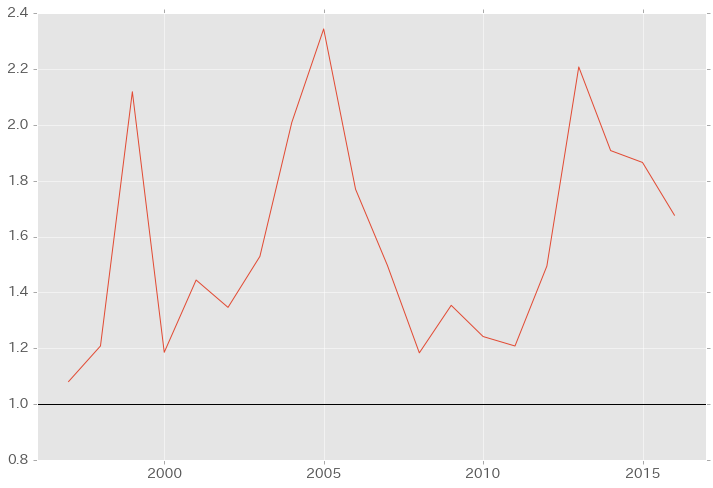
\includegraphics[clip,width=14cm]{/Users/okb/sourcetree/IPO_analysis/paper/latex/transition.png}
    \label{transition}
  \end{center}
\end{figure}

一方で、近年の行動経済学・行動ファイナンスの発展に伴い、プレーヤーの限定合理性を導入してアンダープライシングを説明しようとする研究が展開されている。その代表的なものとして、後の投資家は、それまでの他の投資家が行った購入意思決定を意思決定に反映させ、自らの都合に合わせて情報を無視、あるいは軽視し、先の投資家に追随する、情報カスケード効果\footnote[6]{Welch (1992)\cite{Welch}がその端緒とされている。}が挙げられるだろう。\par

もちろん、現実的な解釈としては、「どの仮説が正しい/誤っている」という話ではなく、それぞれの仮説が折り重なった結果、しているものであるが、

本稿では、図\ref{transition}のように、アンダープライシングの程度が時期によって大きく異なっていることへの説明には不十分である。\par
\subsection{マーケット・センチメントを説明した先行研究の展望}

	
\section{リサーチ・デザイン}
\subsection{データ・ソース}
\subsection{データの特徴}
\subsection{モデルの構造と想定される結果}
\section{実証分析の結果}
\section{総括と今後の課題}

\newpage


\begin{thebibliography}{99}
\bibitem{okamura} 岡村秀夫(2011)「IPO研究の展開」, 『商学論究, 58(3):45-65』
\bibitem{tatsumi} 辰巳憲一・桂山靖代 「IPOリターン・リバーバル —初取引日前後IPOパフォーマンスのアノマリー分析—」, 『学習院大学 経済論集, 第42巻 第3号』
\bibitem{Loughran} Loughram, T., Ritter, J. and Rydqvist, K. (1994) "Initial Public Offering: International Insights," Pacific-Basin Finance Journal 2, 165-199. (updated 2015)
\bibitem{ikeda} 池田直史 (2013) 「IPOの株価観察不能性と正の初期収益率」, 『金融経済研究, 第35号 34-51』
\bibitem{Welch} Welch, I. (1992) "Sequential Sales, Learning, and Cascades," The Journal of FINANCE 47, 695-732.
\end{thebibliography}
\end{document}